\documentclass[twocolumn,prd,superscriptaddress,amsfonts,amssymb,amsmath,preprintnumbers]{revtex4-1}
\usepackage{epsfig}
\usepackage{graphics}
\usepackage{graphicx}
\usepackage{bm}
\usepackage[dvipsnames]{xcolor}
\usepackage{bm}
\usepackage{times}
\usepackage{xspace}
\usepackage[varg]{txfonts}
\usepackage[normalem]{ulem} % To get strikethrough (\sout)
\usepackage[colorlinks]{hyperref}
\usepackage[caption=false]{subfig}
\usepackage{booktabs}
\usepackage{url}
\usepackage{float}



\definecolor{LinkColor}{rgb}{0.75, 0, 0}
\definecolor{CiteColor}{rgb}{0, 0.5, 0.5}
\definecolor{UrlColor}{rgb}{0, 0, 0.75}
\hypersetup{linkcolor=LinkColor}
\hypersetup{citecolor=CiteColor}
\hypersetup{urlcolor=UrlColor}
\usepackage{perpage}
\MakePerPage{footnote}

\newcommand{\paperone}{Paper~I\xspace}
\newcommand{\abhi}[1]{\textcolor{red}{[\textit{AG: #1}]}}
\newcommand{\rb}[1]{\textcolor{blue}{[\textit{RB: #1}]}}

\newcommand{\h}{\mathpzc{h}}
\newcommand{\Hhat}{\hat{\mathpzc{H}}}
\newcommand{\B}{\mathpzc{B}}
\newcommand{\hlm}{\mathpzc{h}_{\ell m}}
\newcommand{\xilm}{\xi_{\ell m}}
\newcommand{\Ylm}{{Y}^{-2}_{\ell m}}
\newcommand{\Y}{{Y}^{-2}}
\newcommand{\hc}{h_\times}
\newcommand{\hp}{h_+}
\newcommand{\Fc}{F_\times}
\newcommand{\Fp}{F_+}
\newcommand{\Mf}{M_f}
\newcommand{\cA}{\mathpzc{A}}
\newcommand{\lm}{_{\ell m}}
\newcommand{\deff}{d_\mathrm{eff}}
\newcommand{\rmi}{\mathrm{i}}
\newcommand{\blambda}{\bm{\lambda}}
\newcommand{\btheta}{\bm{\theta}}
\newcommand{\bxi}{\bm{\xi}}
\newcommand{\bzeta}{\bm{\zeta}}
\newcommand{\bs}[1]{\bm{\vec{s}_{#1}}}
\newcommand{\Mo}{M_{\odot}}
\newcommand{\FFe}{\mathrm{FF}_\mathrm{eff}}
\newcommand{\FF}{\mathrm{FF}}
\newcommand{\e}{\mathrm{e}}
\newcommand{\rhoopt}{\rho_\mathrm{opt}}
\newcommand{\rhosubopt}{\rho_\mathrm{subopt}}
\newcommand{\fqnm}{f}
\newcommand{\sigmaqnm}{\sigma}
\newcommand{\n}{\mathbf{n}}
\newcommand*{\skymapscale}{0.5}
\newcommand*{\paramestscale}{0.455}

\begin{document}

\title{pSEOBNRv4HM}

\author{Abhirup Ghosh}
\affiliation{Max Planck Institute for Gravitational Physics (Albert Einstein Institute), D-14476 Potsdam-Golm, Germany}
\author{Richard Brito}
\affiliation{Dipartimento di Fisica, ``Sapienza" Universit`a di Roma $\&$ Sezione INFN Roma1, Piazzale Aldo Moro 5, 00185, Roma, Italy}
\author{Alessandra Buonanno}
\affiliation{Max Planck Institute for Gravitational Physics (Albert Einstein Institute), D-14476 Potsdam-Golm, Germany}

\date{\today}

\maketitle

%%%%%%%%%%%%%%%%%%%%%%%
% Abstract
%%%%%%%%%%%%%%%%%%%%%%%

\section{Introduction}\label{sec:intro}

\iffalse
Overview of LIGO-Virgo tests of GR
No-hair theorem and overview of nohair and ringdown tests with LIGO-Virgo Observations and future detectors
Describe briefly the test
Motivate the test: full IMR SNR, t0 definition, flexibility
highlight importance of spins
Section breakdown
\fi

The LIGO Scientific Collaboration~\citep{lsc} and the Virgo Collaborations~\citep{Virgo} recently announced their catalogue of gravitational wave observations~\citep{GWTC-2} from the first half of their third observing run~\citep{O3reference}. Combined with the confirmed observations from the first and second observing runs~\citep{abbott2019gwtc}, the Advanced LIGO detectors at Hanford, Washington and Livingston, Louisiana~\citep{aasi2015characterization}, and the Advanced Virgo detector in Cascina, Italy~\citep{acernese2014advanced} have now detected more than $40$ gravitational wave events from the merger of compact objects like neutron stars and/or black holes (compact binary coalescences/CBCs). Alongside independent claims of detections~\citep{nitz20191,nitz20202,2019PhRvD.100b3007Z,2020PhRvD.101h3030V,Venumadhav_2020}, this has firmly established the field of gravitational wave astronomy, five years on from the first ever direct detection of gravitational waves on Earth, on September 14, 2015~\citep{abbott2016observation}. 
\par
Observation of gravitational waves have had significant astrophysical and cosmological implications~\citep{LSC_2016astroph,gw170817_mma,gw170817_joint,gw170817_hubble}. It has also allowed us to make statements in fundamental physics. Specifically, LIGO-Virgo's observations have allowed us to test predictions of Einstein's theory of General Relativity~\citep[GR]{}, in previously unexplored regimes of highly relativistic, strong-field regimes of gravity~\citep{LSC_2016grtests,GW170817_TGR,gwtc1_tgr}. In GR, a CBC involving two black holes (a binary black hole/BBH system) is described in three distinct phases: an early \textit{inspiral}, where the two compact objects spiral in and \textit{plunge} due to a back-reaction of gravitational-wave-emission, a \textit{merger} event marked by the formation of an apparent horizon~\citep{NRpaper}, and a late-time \textit{ringdown}, where the newly formed remnant object settles down to a stable Kerr state through the emission of an exponentially damped quasi-normal-mode (QNM) spectrum of gravitational radiation~\citep{vishu,earlyqnmpapers}.  We have performed tests of gravitational wave generation and source dynamics, where we place bounds on parametrised deviations in the Post-Newtonian coefficients describing the early inspiral~\citep{earlydevelopmentpapers}, and phenomenological coefficients describing the intermediate (plunge) and merger regimes of coalescence~\citep{TIGERmethodspapers}, tests of gravitational wave propagation, which assume a generalised dispersion relation and place upper bounds on the Compton wavelength and consequently, the mass of the graviton~\citep{gw170104,samajdar2017projected} and tests of the polarisation of gravitational radiation using a multi-gravitational-wave-detector network~\citep{gw170814,isi2017probing}. We have also checked for consistency between different portions of the signal using estimates of final mass and spin~\citep{Ghosh:2016xx,Ghosh:2017gfp,LSC_2016grtests}, and consistency of the residuals with interferometric noise~\citep{Ghonge:2020suv,gwtc1_tgr}. None of these tests report any departure from the predictions of GR.
\par
Tests of black hole ringdown and nature of the remnant object is an active field of research at the moment. The no-hair conjecture in GR~\citep{} states that an (electrically neutral) astrophysical black hole is completely described by two observables: mass and spin angular momentum. One consequence of the no-hair conjecture is that the (complex) QNM frequencies of gravitational radiation emitted by a perturbed isolated black hole is uniquely determined by its mass and spin angular momentum. Hence a test of the no-hair conjecture would involve checking for consistency between estimates of mass and spin of the remnant object across multiple QNM frequencies. An inconsistency would either indicate a non-black hole nature of the remnant object, or an incompleteness of GR as a theory of gravity. The consistency between the post-merger signal and the least dampled QNM was first demonstrated in ~\citep{LSC_2016grtests}, and later extended to include overtones in~\citep{Giesler:2019uxc,Isi:2019aib,Bhagwat:2019dtm,Forteza:2020hbw}. Consistency of the late-time signal with a single QNM is a test of the ringdown of a BBH coalescence, but not necessarily a test of the no-hair conjecture, which requires the measurement of (atleast) two QNMs (black hole spectroscopy), and checking for consistency between them. Recent work in that direction include~\citep{Carullo:2018gah,Carullo:2019flw,Bhagwat:2019bwv}. The nature of the remnant object has also been explored through tests of black hole thermodynamics, like the Hawking's area theorem~\citep{Cabero:2017avf} or through search for echos in the post-merger signal~\citep{Nielsen:2018lkf,Tsang:2019zra,Lo:2018sep,Abedi:2018npz,Abedi:2020sgg,Testa:2018bzd}. None of these tests have found evidence for non-black hole nature of the remnant object (as described in GR) in LIGO-Virgo BBH observations.
\par
Most of the tests mentioned above focus on analysing the post-merger or late-time ringdown signal in isolation. Second generation ground-based interferometric detectors like Advanced LIGO and Virgo are most sensitive to stellar-mass black hole binaries that merge near the minima of their sensitivity band ($\sim 100$Hz). As a consequence, the remnant object \textit{rings down} in shot-noise dominated higher frequencies, leaving very little signal-to-noise ratio (SNR) in the post-merger signal. Furthermore, the post-merger signal of a BBH coalescence transitions from a non-linear to a linear regime where the description of the signal as a QNM spectrum becomes appropriate~\citep{}. The ringdown start time isn't a clearly defined quantity and has been explored in detail in~\citep{Bhagwat:2017tkm}. In other works~\citep{Carullo:2018gah,Carullo:2019flw}, it has been left as a free parameter to be estimated directly from the data. Uncertainties in estimates of the ringdown start-time, as well as an overall lack of SNR in the post-merger signal, given typical sensitivities of ground-based detectors result in significant statistical uncertainties in the measurement of the QNM frequencies.
\par
An independent approach to black hole spectroscopy, based on a full-signal analysis, was outlined in~\citep{Brito:2018rfr} (henceforth referred to as \paperone). \abhi{describe underlying GR model; parameterisation; advantages over other methods; highlight spin} 



Unlike methods that focus on the post-merger signal, it describes a framework in which a complete inspiral-merger-ringdown (IMR) waveform model is used to measure the complex QNM frequencies. \abhi{It is a spinning multipolar effective-one-body waveform calibrated to numerical relativity simulations (SEOBNRv4HM~\citep{Cotesta:2018fcv}})This allows access to the full SNR of the signal, reducing measurement uncertainties. Moreover, the definition of the ringdown start time is built into the model and does not need to be either left as an additional free parameter or fixed using alternate definitions. While \paperone presented the method in the context of a non-spinning waveform model, we extend the analysis to the case with black holes spins in the current paper. All astrophysical black holes are expected to be spinning, and ignoring effects of spin have been shown to introduce systematic biases in the measurement of the source properties.
\par
The rest of this paper is organized as follows. Section~\ref{sec:model} describes our parametrised IMR waveform model. In section~\ref{sec:method}, we define our testing GR framework in which we use that model to measure the complex QNM frequencies in a Bayesian formalism. Then in section~\ref{sec:results}, we demonstrate our method on real gravitational wave events, as well as simulated signals. Finally we provide a summary of our results and discuss future developments in section  The rest of this paper is organized as follows. Section~\ref{sec:model} describes our waveform model, which is then used to perform our test of black hole ringdown using Bayesian framwork, outlined in section~\ref{sec:discussion}.

\section{Method}
\subsection{Waveform Model}\label{sec:model}

%\abhi{Summary of the section:}

%\begin{itemize}
%\item{a description of the SEOBNRv4HM model and it's generalisation to form the pSEOBNRv4HM model}
%\item{highlight the importance of spins in the model, especially with regards to the non-spinning method outlined in Brito et al.}
%\end{itemize}

As in \paperone, we use an IMR waveform model developed within the EOB formalism. However, in this work we extend the results of \paperone by using a waveform model for spinning, nonprecessing binary BHs. Namely we use as our baseline model the multipolar waveform developed in Ref.~\citep{Cotesta:2018fcv}. In addition to being calibrated to NR simulations, this model also uses information from BH perturbation theory for the merger and ringdown phases. Therefore this waveform model provides a very accurate and faithful semi-analytic description of the inspiral, merger and ringdown phases. Henceforth we will denote this model by SEOBNR for short.


In the observer's frame, the GW polarizations can be written as 
$h_+(\iota,\varphi;t ) - i h_\times(\iota,\varphi;t) = \sum_{\ell, m} {}_{-\!2}Y_{\ell m}(\iota,\varphi)\, h_{\ell m}(t)$, where $\iota$ denotes the inclination angle computed with respect to the direction perpendicular to the orbital plane, $\varphi$ is the azimuthal direction to the observer, ${}_{-\!2}Y_{\ell m}(\theta,\phi)$ are the $-2$ spin-weighted spherical harmonics. The SEOBNR model we employ includes the $(\ell, |m|)=(2,2),(2,1)$, $(3,3)$, $(4,4)$, and $(5,5)$ modes. For each $(\ell, m)$, the inspiral-(plunge-)merger-ringdown SEOBNR waveform is schematically given by $h_{\ell m}(t) = h_{\ell m}^\mathrm{insp-plunge}\, \theta(t_\mathrm{match}^{\ell m} - t) + h_{\ell m}^\mathrm{merger-RD}\,\theta(t-t_\mathrm{
    match}^{\ell m})$, where $\theta(t)$ is the Heaviside step function, $h_{\ell m}^\mathrm{insp-plunge}$ represents the inspiral-plunge part of the waveform, whereas $h_{\ell m}^\mathrm{merger-RD}$ denotes the merger-ringdown phase. 
  %  
The merger-ringdown SEOBNR modes read~\citep{Bohe:2016gbl,Cotesta:2018fcv}
%
\begin{equation}
  \label{RD}
  h_{\ell m}^\mathrm{merger-RD}(t) = \nu A_{\ell m}(t) e^{i\phi_{\ell m} (t)}\,
  e^{-i\sigma_{\ell m0} (t-t_\mathrm{match}^{\ell m})} \quad t \geq t_{\rm match}^{\ell m}\,,
\end{equation}
%
where $\nu$ is the symmetric mass ratio of the binary and $\sigma_{\ell m0} = \omega_{\ell m 0} -i/\tau_{\ell m 0}$ denotes the complex frequency of the fundamental QNMs of the remnant BH. We denote the oscillation frequencies by $\omega_{\ell m  0}\equiv \Re(\sigma_{\ell m0})$ and the decay times by $\tau_{\ell m 0}\equiv -1/\Im(\sigma_{\ell m0})$. The explicit expressions for the amplitudes $A_{\ell m}(t)$ and phases $\phi_{\ell m} (t)$ can be found in Ref.~\citep{Cotesta:2018fcv}, and are chosen such that the functions $A_{\ell  m}$ and $\phi_{\ell  m}$ are of class $C^1$ at $t=  t_{\rm match}^{\ell m}$, when matching the merger-ringdown waveform to the inspiral-plunge SEOBNR waveform $h_{\ell m}^\mathrm{inspiral-plunge}(t)$.
 
In the SEOBNR model constructed in Ref.~\cite{Cotesta:2018fcv}, the complex frequencies $\sigma_{\ell m 0}$  are expressed in terms of the final BH mass and spin~\cite{Berti:2005ys,Berti:2009kk}, and the latter are related to the BBH's component masses and spins through NR--fitting-formulas obtained in GR~\cite{Taracchini:2013rva,Hofmann:2016yih}. Here instead, in the spirit of what was done in \paperone, we promote the QNM (complex) frequencies to be free parameters of the model, while keeping the inspiral-plunge modes $h_{\ell m}^\mathrm{inspiral-plunge}(t)$ fixed to their GR values (henceforth, pSEOBNR model). We note that when leaving $\sigma_{\ell m}$ to vary freely, the amplitudes $A_{\ell m}(t)$ and phases $\phi_{\ell m} (t)$ will in general also differ from the GR prediction, since those functions depend on the QNM complex frequencies (see~\citep{Cotesta:2018fcv}).

For the specific applications of this paper, we will normally only allow either $\sigma_{220}$ or $\sigma_{330}$ to vary, while keeping all the other modes to coincide with GR. However the model can be easily used to measure any QNM complex frequency available in the waveform.



\subsection{Bayesian PE}\label{sec:method}

A gravitational waveform from the (quasi-circular) coalescence of two black holes is completely described in GR by a set \textit{intrinsic} parameters, $\bxi$: the masses, $m_1, m_2$ and spins, $\bs1, \bs2$ of the initial binary and a reference time and phase $t_c, \phi_c$ respectively; and a set of \textit{extrinsic} parameters, $\btheta$: the location of the binary given by the right ascension, $\alpha$, declination,$\delta$ and the luminosity distance, $d_L$, and its orientation described through the inclination of the binary $\iota$ and its polarisation $\psi$. Also allowing for additional degrees of freedom $\bzeta$ like the complex QNM frequencies described in section \ref{sec:model}, one can then use a Bayesian formalism to obtain a posterior probability density function on the combined parameter set $\blambda = \{\bxi, \btheta, \bzeta\}$:

\begin{equation}
p(\blambda | d, H, I) \propto P(\blambda | H,I) \mathcal{L}(d | \blambda, H, I)
\end{equation}

where $P(\blambda | H,I)$ is the prior probability density function and $\mathcal{L}(d | \blambda, H, I)$ is the likelihood of obtaining the data for a given choice of the parameter set $\blambda$. We assume the hypothesis $H$ to be our waveform model described in section \ref{sec:model} and $I$ to be any other information assumed during the analysis.

Given the full-dimensional posterior probability density function $p(\blambda | d, H, I)$, we can marginalise over the \emph{nuisance} parameters, to obtain the marginalised posterior probability density function on our QNM parameters $\bzeta$, as:

\begin{equation}
p(\bzeta | d, H, I) = \int p(\blambda | d, H, I) d\bxi d\btheta
\end{equation}

Throughout our analysis, we assume the noise in the detector to be well-approximated by the Gaussian random process with a fixed power spectral density. This allows us to define a Gaussian likelihood function $\mathcal{L}(d | \blambda, H, I)$, which we stochastically sample over using either a Markhov-Chain-Monte-Carlo based algorithm implemented in the LIGO Algorithms Library.

\section{Results}\label{sec:results}
\subsection{Priors}

Throughout our analysis we assume a completely uninformed prior in the component masses $m_1, m_2$, uniformly distributed in the range (XX,YY). Our prior on the spins are uniform in the magnitude between (0,1) and isotropic in spin orientation. Our prior on the distance varies as $d_L^2$ upto a distance of XX. For the rest of the parameters we use standard priors as defined in the documentation (CITE Vietch et al. 2015 LALInference paper). For our non-GR ringdown parameters, we assume priors uniform in the range (XX,YY). For $d\tau = -1$, we encounter a singularity (the imaginary part of the frequency goes to infinity), which we avoid by restricting the minimum of the prior on $d\tau$ to be greater than $-1$.

\subsection{Results on GW150914-like injection}


\begin{figure*}
	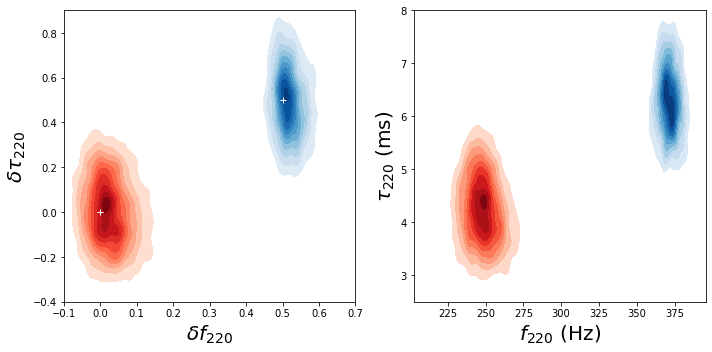
\includegraphics[width=\textwidth]{figures/GW150914_swinj_GR_vs_modGR.png}
	\caption{final figure will contain a third set of contours for modGR recovered assuming GR to show bias. That run is ongoing.}
\end{figure*}

\abhi{The GW150914-like injections we have:}
\begin{itemize}
\item{an SEOBNRv4HM software injection with the 22 mode frequencies estimated}
\item{a non-spinning NR injection with parameters close to the real event but higher SNR for which 22 mode frequencies are estimated}
\item{a non-spinning highly-asymmetric (q=6) NR injection with total mass similar to GW150914 and high SNR for which 22 and 33 mode frequencies are estimated}
\end{itemize}


\subsection{Results on modGR injection}

\abhi{As part of review we had developed the infrastructure to make non-GR waveforms using pSEOBNRv4HM, and running LALInference on it. We had specifically chosen an injection with domega220 = dtau220  = 0.5 in zero-noise, and successfully recovered those frequencies thus demonstrating the robustness of the method in detecting deviations from GR.}

\subsection{Results on actual LIGO-Virgo results}

\begin{figure}
	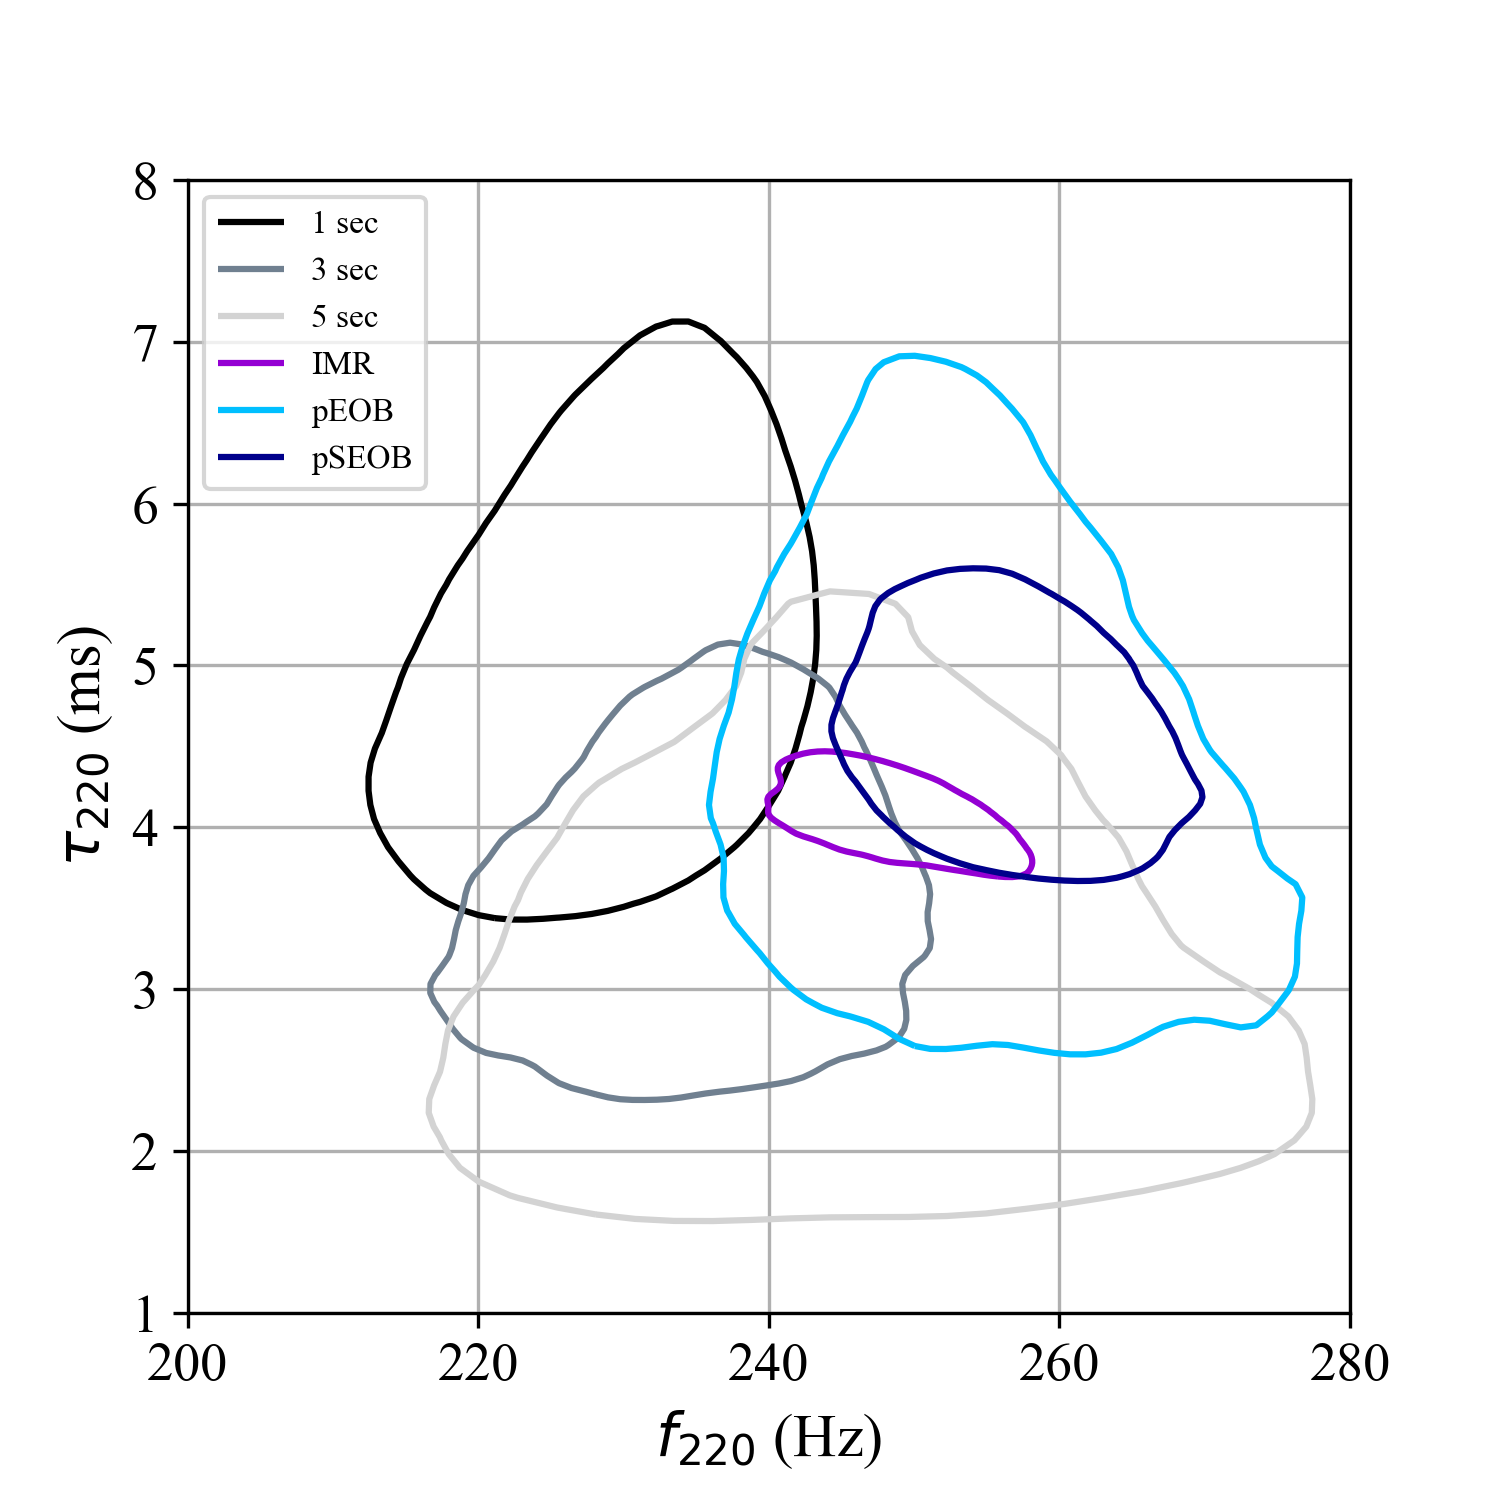
\includegraphics[width=0.4\textwidth]{figures/GW150914.png}
	\caption{include contours from pyRING}
\end{figure}

\abhi{Results obtained as part of the review on GW150914 and other O1-O2 events which are of relevance}
\abhi{A plot showing the fractional quantities}
\abhi{A table with absolute quantites similar to GWTC-2 TGR}

\begin{tabular}{llllllll}
\toprule
Event & \multicolumn{3}{c}{Redshifted} & \hphantom{X} & \multicolumn{3}{c}{Redshifted} \\
& \multicolumn{3}{c}{frequency [Hz]} & \hphantom{X} & \multicolumn{3}{c}{damping time [ms]} \\[0.075cm]
\cline{2-4}
\cline{6-8}
& IMR & DS & pSEOB & \hphantom{X} & IMR & DS & pSEOB \\
\midrule

GW150914 &
$249^{+9}_{-7}$ &
$247^{+14}_{-16}$ &
$-$ &
\hphantom{X} &
$4.1^{+0.3}_{-0.2}$ &
$4.8^{+3.7}_{-1.9}$ &
$-$
\\[0.075cm]

GW170104 &
$286^{+16}_{-27}$ &
$228^{+71}_{-102}$ &
$-$ &
\hphantom{X} &
$3.5^{+0.4}_{-0.3}$ &
$3.6^{+36.2}_{-2.1}$ &
$-$
\\[0.075cm]

GW170729 &
$161^{+13}_{-14}$ &
$148^{+11}_{-11}$ &
$-$ &
\hphantom{X} &
$7.8^{+1.8}_{-1.5}$ &
$10.4^{+8.2}_{-4.7}$ &
$-$
\\[0.075cm]

GW170814 &
$295^{+13}_{-12}$ &
$527^{+340}_{-332}$ &
$-$ &
\hphantom{X} &
$3.7^{+0.3}_{-0.2}$ &
$25.1^{+22.2}_{-19.0}$ &
$-$
\\[0.075cm]

GW170823 &
$199^{+14}_{-16}$ &
$222^{+664}_{-62}$ &
$-$ &
\hphantom{X} &
$5.4^{+1.0}_{-0.6}$ &
$13.4^{+31.8}_{-9.8}$ &
$-$
\\[0.075cm]

\bottomrule
\end{tabular}


\subsection{Results on noise systematics study}

\abhi{A small summary of the noise systematics study that was done for S190521g to show that the deviations seen were consistent with systematics due to noise. The study include 2 separate sections: in Gaussian noise, and in real LIGO-Virgo noise immediately adjacent to the actual event.}

%\begin{figure}[H]
%	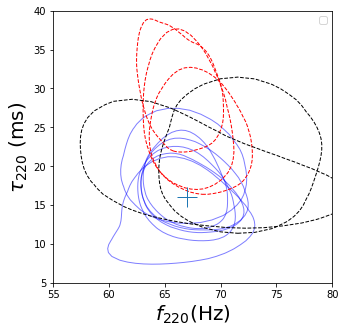
\includegraphics[width=0.4\textwidth]{figures/S190521g_noiseinjections.png}
%	\caption{a single figure for both Gaussian and Real noise injections, color coded, to save space}
%\end{figure}

We injected NRSur7dq4 signal using the MaxL parameters from EXP30, in 2.5 hours of data surrounding the event at: t0-1.5 hours, t0-1., t0-0.5, t0+0.5, t0+1. For 3 of the 5 noise realisations, corresponding to t0-1 hour, t0+0.5 hours, and t0+1.0 hour we recover a damping time similar to the actual event, whereas for a third case, t0-0.5 hours, we obtain a damping time consistent at the 90\% credible interval. L1-SNR goes down by more than 3 in some runs (maximum L1-SNR 12, minimum 9), indicative of how the noise variability is strongly affecting the recovered parameters. For some injections the mass ratio is biased, although final spin (most sensitive to mass ratio) is not affected much.  domega varies quite a lot among runs, instead dtau seems well behaved around zero. Effective frequency is a stable parameter (always well measured), while effective tau is much more sensitive to the noise configuration.  


\section{Discussion}\label{sec:discussion}

\abhi{A comparison with pyRING}
\abhi{damped sinusoid results}

%
\bibliographystyle{apsrev}
\bibliography{intro_paper}

\end{document}